\documentclass[UTF8,a4paper,8pt]{ctexart} 

\usepackage{graphicx}%学习插入图
\usepackage{verbatim}%学习注释多行
\usepackage{booktabs}%表格
\usepackage{geometry}%图片
\usepackage{amsmath}
\usepackage{amssymb}
\usepackage{listings}%代码
\usepackage{xcolor}  %颜色
\usepackage{enumitem}%列表格式
\setenumerate[1]{itemsep=0pt,partopsep=0pt,parsep=\parskip,topsep=5pt}
\setitemize[1]{itemsep=0pt,partopsep=0pt,parsep=\parskip,topsep=5pt}
\setdescription{itemsep=0pt,partopsep=0pt,parsep=\parskip,topsep=5pt}
\usepackage{tcolorbox}
\usepackage{algorithm}  %format of the algorithm
\usepackage{algorithmic}%format of the algorithm
\usepackage{multirow}   %multirow for format of table
\usepackage{tabularx} 	%表格排版格式控制
\usepackage{array}	%表格排版格式控制
\usepackage{hyperref} %超链接 \url{URL}

\CTEXsetup[format+={\flushleft}]{section}

%%%% 设置图片目录
\graphicspath{{figure/}}

%%%% 段落首行缩进两个字 %%%%
\makeatletter
\let\@afterindentfalse\@afterindenttrue
\@afterindenttrue
\makeatother
\setlength{\parindent}{2em}  %中文缩进两个汉字位

%%%% 下面的命令重定义页面边距,使其符合中文刊物习惯 %%%%
\addtolength{\topmargin}{-54pt}
\setlength{\oddsidemargin}{0.63cm}  % 3.17cm - 1 inch
\setlength{\evensidemargin}{\oddsidemargin}
\setlength{\textwidth}{14.66cm}
\setlength{\textheight}{24.00cm}    % 24.62

%%%% 下面的命令设置行间距与段落间距 %%%%
\linespread{1.4}
\setlength{\parskip}{0.5\baselineskip}
\geometry{left=1.6cm,right=1.8cm,top=2cm,bottom=1.7cm} %设置文章宽度
\pagestyle{plain} 		  %设置页面布局

%代码效果定义
\definecolor{mygreen}{rgb}{0,0.6,0}
\definecolor{mygray}{rgb}{0.5,0.5,0.5}
\definecolor{mymauve}{rgb}{0.58,0,0.82}
\lstset{ %
	backgroundcolor=\color{white},   % choose the background color
	basicstyle=\footnotesize\ttfamily,      % size of fonts used for the code
	%stringstyle=\color{codepurple},
	%basicstyle=\footnotesize,
	%breakatwhitespace=false,         
	%breaklines=true,                 
	%captionpos=b,                    
	%keepspaces=true,                 
	%numbers=left,                    
	%numbersep=5pt,                  
	%showspaces=false,                
	%showstringspaces=false,
	%showtabs=false,        
	columns=fullflexible,
	breaklines=true,                 % automatic line breaking only at whitespace
	captionpos=b,                    % sets the caption-position to bottom
	tabsize=4,
	commentstyle=\color{mygreen},    % comment style
	escapeinside={\%*}{*)},          % if you want to add LaTeX within your code
	keywordstyle=\color{blue},       % keyword style
	stringstyle=\color{mymauve}\ttfamily,     % string literal style
	frame=single,
	rulesepcolor=\color{red!20!green!20!blue!20},
	% identifierstyle=\color{red},
	language=c++,
}

 \author{\kaishu 郑华}
 \title{DirectX 笔记}
 
 %正文排版开始
\begin{document} 
 	\maketitle
	\tableofcontents
\newpage
\section{学习地址}\url{http://www.directxtutorial.com/default.aspx}
 
\section{下载安装}
  DirectX 是一个代码库集合,提供给游戏和多媒体应用一个公共的函数集合
  
\section{创建DirectX3D窗口}
 
	 怎样创建一个工程
	 
	 怎样建立窗口程序
	 
	 怎样初始化 DirectX
	 
	 怎样清除屏幕(清屏)
	 
	 怎样显示场景
 
	 \paragraph{问题:stdafx.h  to resuorces }:
		 在导入的头文件们的\underline{最前面}加上
		 \verb|#include "stdafx.h"|
	 \paragraph{问题:unresolved external symbol \_DXTraceW@20 referenced in function}
		 需要链接 库\verb|d3d11.lib, d3dx11.lib, dxerr.lib|,还有就是
		 在 添加库时只添加 lib--x86,不管是64位还是32位都是添加x86,因为编写的程序位win32
 
	 \paragraph{问题:DirectX clear函数 不起作用,即不改变窗口颜色}:
		 使用win32 默认的消息循环,导致进入不了绘图方法
	 
	 \paragraph{问题:Access 0x00000} 
		 数组变量未初始化,指针未初始化等。
 
 \newpage
 \section{绘制流水线-四大变换}
	 \subsection{绘制变换概述}
		 空间中的物体是3维的,而显示屏是2维的,所以需要将物体的空间三维坐标变换为二维坐标,俗称“顶点坐标变换”,接着如图显示生活中的光照是万物皆需要的,光照处理,接着光栅化处理,最后成像显示。
	 
		 总体如图所示:
		  \begin{figure}[h]
		  	\centering
		  	\includegraphics[angle=0,width=8cm]{introduce.jpg}%就在前面括号中写图片名
		  	\caption{转换概述原理}
		  	\label{fig:gaishu}
		  \end{figure}%
 
			  1- 世界变换:摆好带拍摄的物品或人物 ,为了能在世界空间中指定位置来绘制图形
	  
			  2- 取景变换:调整好拍摄角度,为了以不同的视角观察图形
	  
			  3- 投影变换:调整焦距:正交投影,透视投影,为了将相对较远的图形投影到同一个平面上并体现近大远小的真实视觉效果
				    \begin{figure}[h]
				    	\centering
				    	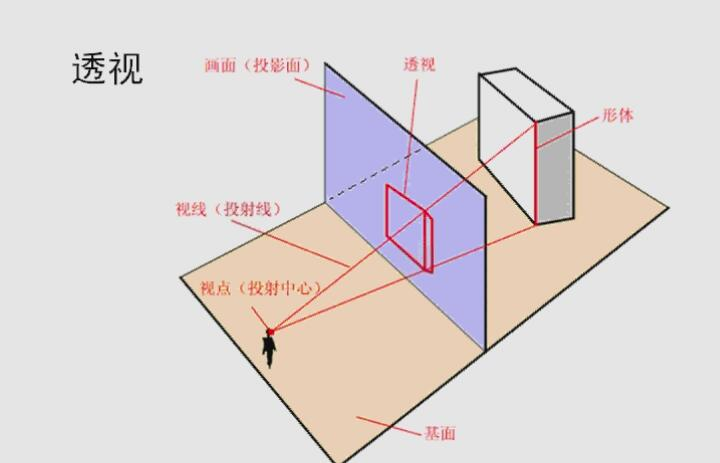
\includegraphics[angle=0,width=8cm]{TouShi.jpg}%就在前面括号中写图片名
				    	\caption{透视图原理}
				    	\label{fig:Toushi}
				    \end{figure}%
  
			  4- 拍摄或视口变换:为了控制显示图形的窗口的大小,比例以及深度等信息      
			  
				   \begin{figure}[h]
					   	\centering
					   	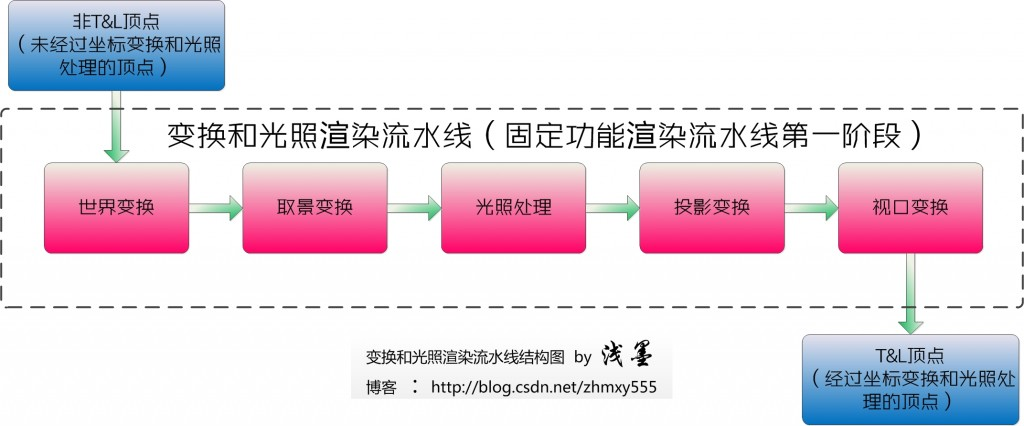
\includegraphics[angle=0,width=8cm]{ChangeOfPointMatrix.jpg}%就在前面括号中写图片名
					   	\caption{转换第一阶段}
					   	\label{fig:zhuanhuan}
				   \end{figure}%
	\subsection{世界变换}
		根据物体模型的大小、方向以及其他模型之间的相对关系,世界变换将物体模型从自身的局部坐标系中转换到时间坐标系中
	
	\subsection{取景变换}
		也就是设置Direct3D中的虚拟摄像机的位置和观察点。对于处于不同位置的虚拟摄像机和观察点,其观察物体模型的视角方向也有所差异,因此实际看到的物体模型的实际形状也有所不同。正所谓“横看成岭侧成峰”,就像这幅图所传达的观点一样
	
	\subsection{投影变换}
		经过上一步的取景变换之后,物体模型就位于观察坐标系中了,然而为了能够将三维场景显示在我们二维的显示平面上(因为我们的显示屏是二维的),还需要通过投影变换将三维物体投影到二维的平面上,这个过程我们就把它叫做透视投影
	
	\subsection{视口变换}
		视口变换用于将投影窗口中的图形转换到显示屏幕的程序窗口中。视口是程序窗口中前的一个矩形区域,他可以是整个程序窗口,也可以是窗口的客户区,也可以是窗口中其他矩形区域
\newpage
\section{画图}
		\paragraph{函数原型}\textbf{HRESULT DrawIndexedPrimitive(D3DPRIMITIVETYPE, INT BaseVertexIndex,UINT MinVertexIndex, UINT NumVertices, UINT startIndex,UINT primCount)}
		
			\subparagraph{1 D3DPRIMITIVETYPE}:
			
			Triangle List		
				\begin{figure}[h]
					\centering
					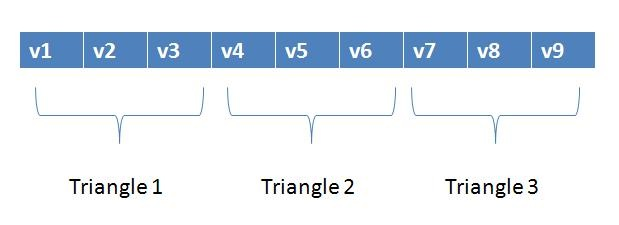
\includegraphics{TriangleList.jpg}
					\caption{TriangleList  Type}
				\end{figure}	
			
			Triangle Strip	
				\begin{figure}[h]
					\centering
					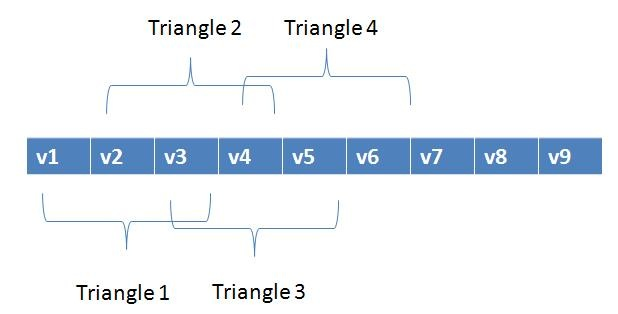
\includegraphics{TriangleStrip.jpg}
					\caption{TriangleSrip  Type}
				\end{figure}
				
			\subparagraph{2 BaseVertexIndex}
				顾名思义,初始顶点索引。注意,这里的“索引”与绘制图形需要的索引不一样,它这里专指从顶点缓冲中的“第几个”开始获取顶点数据。因为每次取4个,所以对于第i次绘制来说,应该设置为i*4。例如,i=1时,即从顶点缓冲区中第4个顶点开始获取顶点数据
			
			\subparagraph{3 MinVertexIndex}
				顾名思义,最小顶点索引。注意,这里的“索引”与绘制图形需要的索引一样。也就是说,这里设置当前最小的顶点在索引缓冲区中所对应的索引值。例如,对于i=1来说,从顶点缓冲区中第4个顶点开始获取顶点数据,获取4个顶点,则得到的顶点数据分别是4,5,6,7;如果这个时候设置最小顶点索引为0,则第4个顶点在索引缓冲区中对应的索引值是0,第5个顶点则对应索引值1,6对应2,7对应3.
			
			\subparagraph{4 NumVertices}
				顾名思义,顶点个数。这里的顶点个数,是本次绘制需要从顶点缓冲区获取的顶点个数。本例中,是4,即每次绘制需要获取4个顶点
			
			\subparagraph{5 StartIndex}
				顾名思义,开始的索引值。本例设置为0,即从索引缓冲区中的第0个索引开始
			
			\subparagraph{6 PrimCount}
				顾名思义,本次绘制的图元个数。本例中设置为2,即绘制2个三角形组成一个面
			
			\subparagraph{Use And Analysis}:
				\begin{lstlisting}
	for(int i = 0; i < 6; i++)
	{
		m_pD3DDevice->DrawIndexedPrimitive(D3DPT_TRIANGLEFAN, i * 4, 0, 4, 0, 2);
	}				 
				\end{lstlisting}
				
				\begin{enumerate}[fullwidth,itemindent = 2em]
					\item 从顶点缓冲区中的第i*4个顶点开始,获取4个顶点数据
					\item 最小顶点索引是0,所以获取的4个顶点的索引依次是0,1,2,3
					\item 然后从索引缓冲区的第0个索引开始,获取4个索引
					\item 然后根据这4个索引值,根据三角形扇,绘制2个三角形,组成一个面
					\item 绘制6次,生成6个面
				\end{enumerate}
			\subparagraph{参考位置}:
			
			\url{http://blog.sina.com.cn/s/blog_5a6f39cf01016jax.html}  //Function Introduce
		
		    \url{http://www.cnblogs.com/graphics/archive/2012/07/21/2603041.html}   //Types
		    
		    \subparagraph{Note}:
			    只有在调用 Present时才会更新屏幕
			    
	\subsection{错误记录}			   	    
		\paragraph{画图连原点错误}:
				该错误出现的情况大多数如下所图示,将最后一个三角行与原点连接起来..
					\begin{figure}[h]
						\centering
						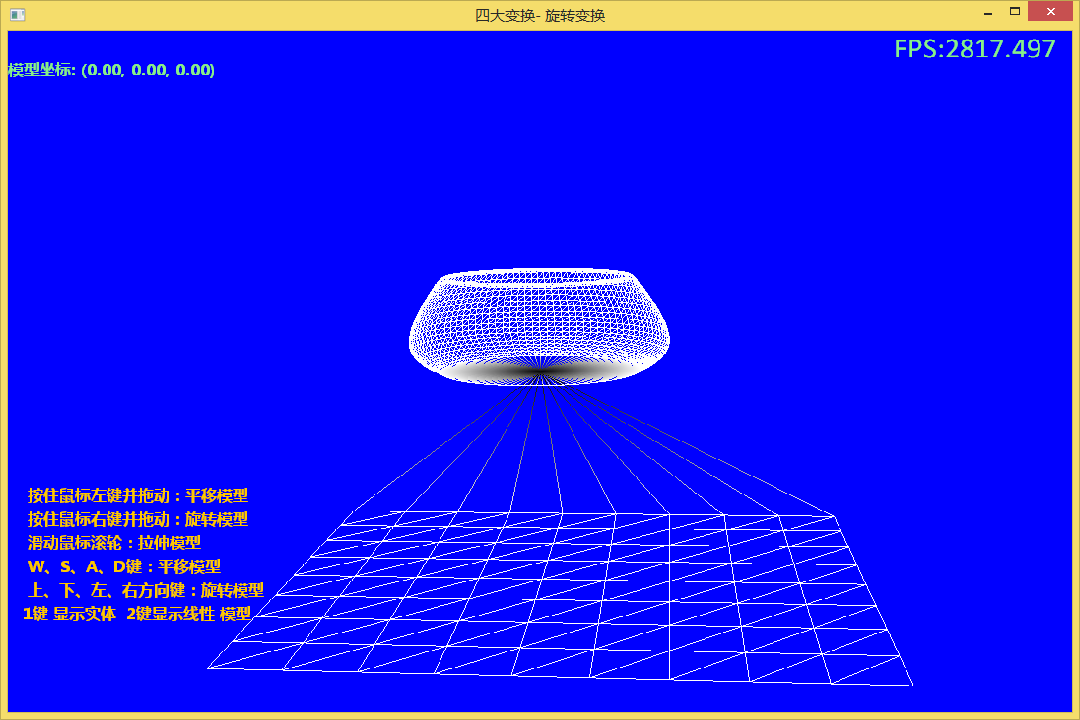
\includegraphics[angle=0,width=12cm]{Error-Point.png}
						\caption{连原点  Type}
					\end{figure}
				 \subparagraph{错误原因}:给的点数少于实际花三角形所需要的点数,这时从构造点处找错误	
				
\newpage
\section{光照}
	\paragraph{1.光照类型}
		\subparagraph{环境光 Ambient Light}
			这种类型的光是指光源发出的光经过其他物体表面反射而到底该物体表面的光。物体没有被光源直接照射
		\subparagraph{漫射光 Diffuse Light}
			这种类型的光沿特定方向传播,到达某一表面时将沿着各个方向均匀反射(即物理中的漫射
		\subparagraph{镜面光 Specular Light}
			这种类型的光沿特定方向传播,到达一个表面后将严格地反射,所以只能在某一个角度内看到高亮度照射
			
	\paragraph{2.材质}
		\subparagraph{定义}
			 在现实世界中,我们观察到物体的颜色实际上由该物体反射出的光的颜色决定的。因此,当一个红色的球体受到红光(只要包含红光成分即可)的照射,则呈现出红色;但是如果用蓝光照射该红色球体,则我们无法观测到这个球体,因为它吸收了全部的蓝光而不反射任何光,它对于我们而言是“黑色”的
		\subparagraph{D3DMATERIAL9 定义材质}:
			\begin{lstlisting}
	//D3DMATERIAL9结构  
	typedef struct D3DMATERIAL9{  
		D3DCOLORVALUE Diffuse;  //对漫射光的反射率  
		D3DCOLORVALUE Ambient;  //对环境光的反射率  
		D3DCOLORVALUE Specular; //对镜面光的反射率  
		D3DCOLORVALUE Emissive; //用于增强物体的亮度  
		float  Power;       //指定镜面高光点的锐度  
	} D3DMATERIAL9,*LPD3DMATERIAL9;  			
			\end{lstlisting}
		\subparagraph{3.顶点法线}
			  Direct3D需要确定顶点法线方向,以便确定光线到达表面的入射角。光照是对每个顶点进行计算的,所以每个顶点都需要知道法线方向。基于此,需要在顶点结构中增加表示顶点法线的属性。
		\subparagraph{4.光源}
			\begin{enumerate}[fullwidth, itemindent = 3em]
				\item 点光源(Point Lights)该光源在世界坐标系有固定的位置,向所有方向发射光线
				\item 方向光(Directional Lights)该光源没有位置信息,发射的光线相互平行地沿某一个特定方向传播
				\item 聚光灯(Spot Lights)该光源有位置信息,发射的光呈锥形并沿着特定方向传播。
			\end{enumerate}
			
				\begin{lstlisting}
	//D3DLIGHT9结构  
	typedef struct D3DLIGHT9{  
		D3DLIGHTTYPE Type;      	//光源类型  
		D3DCOLORVALUE Diffuse;      //漫射光颜色  
		D3DCOLORVALUE Specular;     //镜面光颜色  
		D3DCOLORVALUE Ambient;      //环境光颜色  
		D3DVECTOR Position; 		//光源在世界坐标系中的位置  
		D3DVECTOR Direction;		//光在世界坐标系中传播的方向  
		float Range;        		//光在“消亡”前所能达到的最大光程  
		float Falloff;     			//用于聚光灯  
		float Attenuation0; 		//衰减变量,定义了光强随距离衰减的方式  
		float Attenuation1;  
		float Attenuation2;  
		float Theta;        		//用于聚光灯,指定内部锥形的圆锥角  
		float Phi;      			//用于聚光灯,指定外部锥形的圆锥角  
	} D3DLIGHT9, *LPD3DLIGHT;			  
				\end{lstlisting}
\newpage
\section{纹理与映射}
	\paragraph{总览}
		 在Direct3D中,借助纹理映射(texture mapping)技术可将图像数据映射到三角形单元,从而显著地所绘制图景的细节和真实感。纹理用接口IDirect3DTexture9来表示。纹理类似于表面的一个像素矩阵,与表面不同的是它可被映射到三角形单元
		 
	\paragraph{1.纹理坐标}
		Direct3D所用的纹理坐标系有沿着水平方向的u轴和沿垂直方向的v轴(竖直向下)构成。用坐标对(u,v)标识的纹理元素称为纹理元(texel)。另外,Direct3D为了处理不同尺度的纹理,Direct3D将纹理坐标进行了规范化,使之限定在[0,1]之间。
		
			\begin{figure}[h]
				\centering
				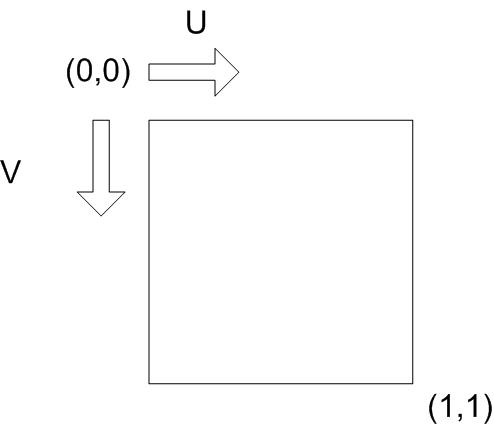
\includegraphics[width = 8cm]{TexturePoints.jpg}
			\end{figure}
		
		 对于每个3D三角形单元,都可以在纹理中定义一个相应的三角形区域,然后将该三角形内的纹理映射到该3D三角形单元中。另外,为实现该映射,需要在顶点结构Vertex中添加纹理坐标,并且设定相应的顶点格式FVF
		 \begin{lstlisting}
	const DWORD Vertex::FVF = D3DFVF_XYZ | D3DFVF_NORMAL | D3DFVF_TEX1; 
		 \end{lstlisting}
		 现在,由3个顶点对象构成的每个三角形都在纹理坐标系中定义了一个相应的纹理三角形
	
	\paragraph{2.创建并启用纹理}
			\subparagraph{创建纹理}:
				 \begin{lstlisting}
	IDirect3DTexture9 * _stonewall;     //创建纹理对象  
	D3DXCreateTextureFromFile(_device, "stonewall.bmp", &_stonewall);   //加载纹理图片 				  
				 \end{lstlisting}
			\subparagraph{设置当前工作纹理}:
				 \begin{lstlisting}
	Device->SetTexture(0, _stonewall);   //设置当前工作纹理  				  
				 \end{lstlisting}
				 \verb|SetTexture(DWORD stage, IDiretct3DBaseTexture9 * pTexture)|函数用于设置当前工作纹理,stage标识纹理层数(Direct3D最多可设置8层纹理,0~7,称为多重纹理),pTexture是纹理指针(为0时表示禁用该层纹理)。
				 
	\paragraph{3.纹理过滤器 OR 多级渐进纹理}
			当纹理最终被映射到屏幕空间中时,由于纹理三角形和屏幕三角形大小的不一致可能导致显示的图像畸变。为克服这种畸变,使用纹理过滤技术(filtering)。
				
			 Direct3D使用三种类型的纹理过滤器,每种过滤器提供一种质量水平,质量越高,开销越大,速度越慢。过滤方式由方法IDirect3DDevice->SetSamplerState来设置。
				  
			 过滤方式:
				  \begin{enumerate}[fullwidth, itemindent = 3em]
					  \item 最近点采样(nearest point sampling)  Direct3D默认过滤方式,处理速度最快,质量最差
					  \item 线性纹理过滤(linear filtering)   效果好,速度较快
					  \item 各向异性纹理过滤(anisotropic filtering)   效果最好,速度最慢
				  \end{enumerate}
				  
			\subparagraph{多级渐进纹理}:同纹理过滤器一样,我们也可以使用多级渐进链(chain of mipmap)消除尺寸畸变
				  
				  具体方法是:由某一纹理创建一系列分辨率逐渐减小的纹理图像,并且对每种分辨率下的纹理所采用的过滤方式进行定制,以便保留较为重要的细节。如下图:
				    \begin{figure}[h]
					  	\centering
					  	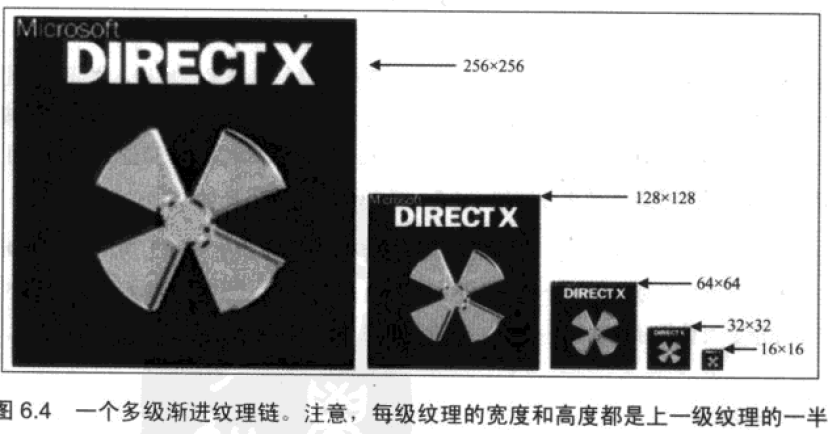
\includegraphics[width=12cm]{Texture.png}
					  \end{figure}
					  
				  多级渐进纹理过滤器主要用于控制Direct3D使用多级渐进纹理的方式。多级渐进纹理过滤器设置函数如下
				  \begin{lstlisting}
	Device->SetSamplerState(0, D3DSAMP_MIPFILTER, Filter); 
				  \end{lstlisting}
				  
				  其中,Filter可取如下值
				  \begin{enumerate}[fullwidth, itemindent = 3em]
				  	\item  D3DTEXF\_NONE   禁用多级渐进纹理过滤器
				  	\item  D3DTEXF\_POINT  将选择尺寸与屏幕三角形最接近的那一级纹理.一旦选择了某一级纹理,Direct3D就会用指定的放大过滤器或者缩小过滤器对该级纹理进行过滤
				  	\item  D3DTEXF\_LINEAR 将选择尺寸与屏幕三角形最接近的两级纹理级,用指定大小的过滤器进行过滤,然后再将这两级纹理进行线性组合,形成最终的颜色值
				  \end{enumerate}
	\paragraph{4.示例}
			\subparagraph{步骤总结}:
				\begin{enumerate}
					\item 构造组成物体的顶点格式, 并为其指定纹理坐标 
					\item 用函数D3DXCreateTextureFromFile为IDirect3DTexture9接口加载一种纹理
					\item 设置缩小过滤器、放大过滤器和多级渐进纹理过滤器
					\item 绘制物体前,用函数IDirect3DDevice9::SetTexture来设定与物体相关联的的纹理
				\end{enumerate}
			\subparagraph{示例代码}:
				\begin{lstlisting}
	IDirect3DVertexBuffer9 * Quad = 0;  
	IDirect3DTexture9 *      Tex  = 0;
	const DWORD Vertex::FVF = D3DFVF_XYZ | D3DFVF_NORMAL | D3DFVF_TEX1;  
	//  
	// 创建顶点缓存  
	//  
	Device->CreateVertexBuffer(  
	6 * sizeof(Vertex),   
	D3DUSAGE_WRITEONLY,  
	Vertex::FVF,  
	D3DPOOL_MANAGED,  
	&Quad,  
	0);  
	
	Vertex* v;  
	Quad->Lock(0, 0, (void**)&v, 0);  
	//两个三角形的顶点坐标以及纹理坐标  
	//用于构建四边形  
	v[0] = Vertex(-1.0f, -1.0f, 1.25f, 0.0f, 0.0f, -1.0f, 0.0f, 1.0f);  
	v[1] = Vertex(-1.0f,  1.0f, 1.25f, 0.0f, 0.0f, -1.0f, 0.0f, 0.0f);  
	v[2] = Vertex( 1.0f,  1.0f, 1.25f, 0.0f, 0.0f, -1.0f, 1.0f, 0.0f);  
	
	v[3] = Vertex(-1.0f, -1.0f, 1.25f, 0.0f, 0.0f, -1.0f, 0.0f, 1.0f);  
	v[4] = Vertex( 1.0f,  1.0f, 1.25f, 0.0f, 0.0f, -1.0f, 1.0f, 0.0f);  
	v[5] = Vertex( 1.0f, -1.0f, 1.25f, 0.0f, 0.0f, -1.0f, 1.0f, 1.0f);  
	
	Quad->Unlock();  
	
	//  
	//创建纹理并设置过滤器  
	//  
	D3DXCreateTextureFromFile(  
	Device,  
	"dx5_logo.bmp",  
	&Tex);  
	
	Device->SetTexture(0, Tex);  
	
	Device->SetSamplerState(0, D3DSAMP_MAGFILTER, D3DTEXF_LINEAR);   //设置放大过滤器为线性  
	Device->SetSamplerState(0, D3DSAMP_MINFILTER, D3DTEXF_LINEAR);   //设置缩小过滤器为线性  
	Device->SetSamplerState(0, D3DSAMP_MIPFILTER, D3DTEXF_POINT);    //设置纹理渐进过滤器  
	
	//  
	//不使用光照  
	//  
	Device->SetRenderState(D3DRS_LIGHTING, false);  
	
	//  
	//设置投影矩阵  
	//  
	D3DXMATRIX proj;  
	D3DXMatrixPerspectiveFovLH(  
	&proj,  
	D3DX_PI * 0.5f, // 90 - degree  
	(float)Width / (float)Height,  
	1.0f,  
	1000.0f);  
	Device->SetTransform(D3DTS_PROJECTION, &proj);				      
				\end{lstlisting}
				  
\newpage
\section{游戏结构}
	  \paragraph{1.游戏引擎部分}
		  通常,最好是将无关的系统分割成不同的动态链接库(DLL),这样可以更方便地将改动过的软件更新、修改和重新发布给用户。如果有任何类型的更新,那么将全部.exe文件重新发布给已经购买该款游戏的用户很不经济。只要开发人员重新发布一个动态链接库(DLL)(只是整个语系中的一小部分),那么效率将会提高很多。虽然现在的宽带Internet使得下载更新信息的速度比过去快很多,但目前所发布的这些游戏远比过去的要庞杂的多。现在的某些游戏仅为了安装在用户的机器上就要用掉4张光盘或更多。这使得在Internet上重新发布整个游戏,效率变得低下。这对用于修复在用户机器上产生严重问题的程序缺陷的主要更新信息而言,是非常可怕的事情。
	  
	  \paragraph{2.游戏项目部分}
	  
\section{脚本系统}
	\paragraph{1.存在的目的与作用}
		在解决复杂问题时,C++程序结构的复杂性和逻辑实现的复杂性,给程序员对程序的改进和维护带来了很大的麻烦。而C++与Lua的结合,让C++可以只负责为lua提供各种基本的功能函数库,而Lua调用这些库来实现各种逻辑功能。这种分工可以让程序员将程序中的基本代码库和逻辑实现代码进行分离,使程序的效率和可维护有了很大的提高。
		
		简单的说,就是将剧情与功能分离, 这样在需要改变剧情时,不用再对源代码进行编译,而只是修改脚本即可。
  
\end{document} 
 		    